\chapter{INTRODUCTION}
\label{chap:1}

\section{Background}
\label{sec:background}

Cardiovascular disease (CVD) remains the leading cause of mortality and
morbidity worldwide \citep{WHO2021,Tsao2022}, with coronary heart disease (CHD) accounting for a
substantial proportion of cardiovascular-related deaths. Among the
various manifestations of CHD, myocardial infarction (MI) represents one
of the most critical cardiovascular conditions because prolonged
interruption of coronary blood flow causes irreversible myocardial
injury, leading to myocardial necrosis, fibrotic scar formation,
ventricular remodeling, impaired cardiac function, and increased
mortality. Consequently, accurate assessment of myocardial infarction is
essential for determining disease severity, therapeutic planning, risk
stratification, and long-term prognosis \citep{Thygesen2019}.

In Indonesia, cardiovascular disease also represents a major healthcare
challenge. According to the Indonesian Ministry of Health \citep{Kemenkes2021},
cardiovascular disease accounts for one of the largest healthcare
expenditures under the National Health Insurance (JKN) program. This
increasing disease burden highlights the need for reliable, objective,
and efficient technologies that can support clinical decision-making
while improving the consistency and reproducibility of cardiac image
analysis.

Cardiac Magnetic Resonance (CMR) has become the reference imaging
modality for myocardial infarction assessment because it provides
excellent soft-tissue contrast, high spatial resolution, and
comprehensive visualization of both cardiac anatomy and myocardial
pathology without exposing patients to ionizing radiation \citep{Kim2000,Kramer2020}. Different CMR sequences provide
complementary diagnostic information. Cine CMR enables accurate
visualization of cardiac structures and ventricular function, whereas
Late Gadolinium Enhancement (LGE) imaging accurately identifies
infarcted and fibrotic myocardial tissue. The combination of these
imaging sequences enables comprehensive assessment of myocardial
infarction from both anatomical and pathological perspectives. The
overall workflow of the proposed framework developed in this
dissertation is illustrated in Figure~\ref{fig:ch1-proposed}. The framework integrates cardiac structure segmentation, reliable myocardium
segmentation, myocardial scar segmentation, and quantitative scar
assessment to support comprehensive myocardial infarction assessment.


\begin{figure}[htbp]
	\centering
	\fbox{\parbox{0.82\textwidth}{\centering Insert Figure 1.1 here}}
	\caption{Overview of the Proposed Deep Learning Framework for CMR Image Analysis for Myocardial Infarction Assessment}
	\label{fig:ch1-proposed}
\end{figure}

Reliable myocardial infarction assessment cannot be achieved directly
from scar segmentation alone. Since myocardial scar is anatomically
confined within the myocardium, accurate cardiac structure segmentation
provides the anatomical foundation for subsequent pathological analysis.
Reliable myocardium segmentation subsequently defines the region of
interest for scar localization, while accurate scar segmentation enables
quantitative assessment of myocardial scar extent. Because these stages
are sequentially connected, errors introduced during earlier analyses
may propagate to subsequent stages and reduce the reliability of the
final assessment.

Despite the superior capability of CMR, image interpretation in routine
clinical practice remains largely dependent on manual image analysis
performed by experienced cardiologists and radiologists. Manual analysis
is time-consuming and susceptible to intra-observer and inter-observer
variability, particularly when myocardial boundaries are indistinct or
scar tissue exhibits heterogeneous signal intensity. These limitations
motivate the development of automated image analysis methods capable of
providing more objective, consistent, and efficient myocardial
infarction assessment.

Recent advances in deep learning have significantly improved medical
image segmentation, including CMR image analysis. Encoder-decoder
architectures, particularly U-Net and its variants, have demonstrated
excellent performance for cardiac structure segmentation, whereas
residual learning, attention mechanisms, and improved improved learning
strategies have further enhanced segmentation accuracy across various
medical imaging applications \citep{Ronneberger2015,He2016,Oktay2018}. Nevertheless, several methodological challenges
remain.

First, preservation of fine anatomical information during cardiac
structure segmentation remains challenging because repeated
down-sampling operations may reduce spatial resolution and boundary
continuity. Second, reliable myocardium segmentation is still affected
by class imbalance and ambiguous myocardial boundaries, requiring
effective learning strategies during network training. Third, myocardial
scar segmentation remains difficult because scar tissue generally
occupies only a small portion of the myocardium while exhibiting
heterogeneous signal intensity and irregular morphology. Finally,
although numerous studies have reported improvements in individual image
analysis tasks, these studies generally investigate each task
independently rather than integrating them into a unified framework for
myocardial infarction assessment.

The research gaps identified from previous studies are illustrated in
Figure~\ref{fig:ch1-fishbone} and summarized in Table~\ref{tab:ch1-tab1_1}. Although considerable progress has been achieved in individual image analysis
tasks, these studies generally address each component independently
rather than integrating them into a unified framework for myocardial
infarction assessment.

\begin{figure}[htbp]
	\centering
	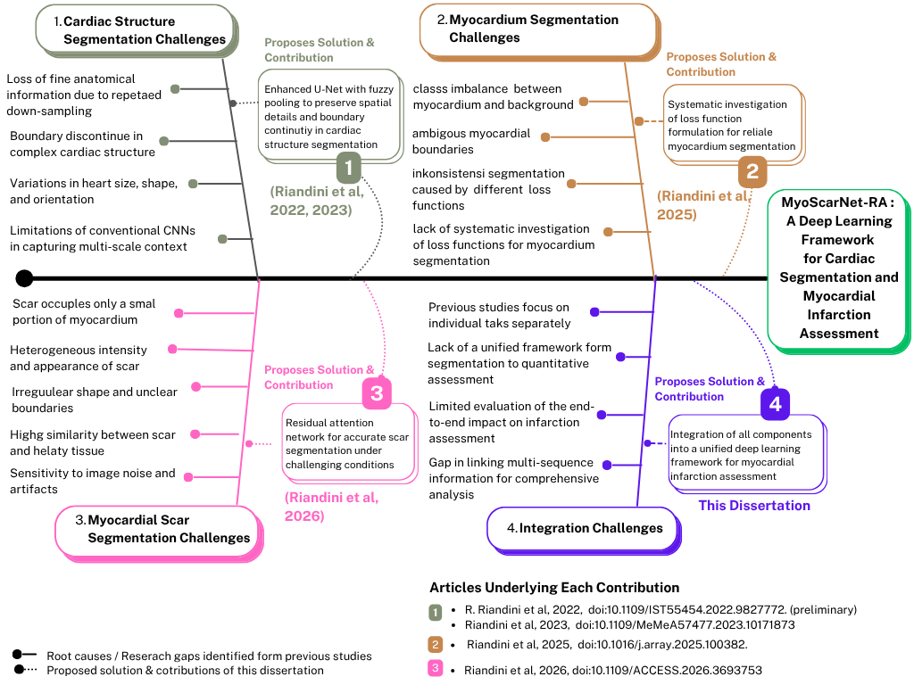
\includegraphics[width=0.86\textwidth]{bab1/ch1-fishbone.png}
	\caption{Fishbone analysis of research challenges in CMR analysis for MI assessment and the proposed solutions with corresponding contributions of this dissertation}
	\label{fig:ch1-fishbone}
\end{figure}

Table 1.1. Research Gap Analysis and Positioning of the Proposed
Dissertation

\begin{longtable}[]{@{}
		>{\raggedright\arraybackslash}p{(\columnwidth - 4\tabcolsep) * \real{0.2444}}
		>{\raggedright\arraybackslash}p{(\columnwidth - 4\tabcolsep) * \real{0.2782}}
		>{\raggedright\arraybackslash}p{(\columnwidth - 4\tabcolsep) * \real{0.4774}}@{}}
	\toprule
	\textbf{Previous Studies} & \textbf{Remaining Limitation} & \textbf{Position of This Dissertation} \\
	\midrule
	\endhead
	
	Cardiac structure segmentation & Focused on anatomical segmentation & Enhanced U-Net with fuzzy pooling \\
	Myocardium segmentation & Investigated independently & Reliable myocardium segmentation through loss function investigation \\
	Myocardial scar segmentation & Focused only on scar segmentation & Residual attention-based scar segmentation with quantitative assessment \\
	Individual image analysis tasks & Conducted separately & Integrated deep learning framework for myocardial infarction assessment \\
	\bottomrule
	\label{tab:ch1-tab1_1}
\end{longtable}

Motivated by these challenges, this dissertation develops an integrated
deep learning framework for CMR image analysis. The proposed framework
consists of four complementary stages: \textbf{(1)} cardiac structure
segmentation using an enhanced U-Net incorporating fuzzy pooling,
\textbf{(2)} reliable myocardium segmentation through systematic
investigation of different loss function formulations, \textbf{(3)}
residual attention-based myocardial scar segmentation followed by
quantitative scar assessment, and \textbf{(4)} integration of these
methodological developments into a unified framework for automated
myocardial infarction assessment. Through this integrated approach, the
dissertation establishes a coherent methodological pathway from
anatomical cardiac representation to quantitative myocardial scar
assessment, providing a comprehensive approach for CMR image analysis.

\section{Research Problems}
\label{sec:research-problems}

Based on the background presented in the previous section, several
research problems remain to be addressed in CMR image analysis for
myocardial infarction assessment. These research problems are formulated
as follows.

\begin{enumerate}
	\def\labelenumi{\arabic{enumi}.}
	\item
	How can cardiac structure segmentation be improved while preserving
	important anatomical information from CMR images?
	\item
	How can reliable myocardium segmentation be achieved under class
	imbalance and ambiguous myocardial boundaries?
	\item
	How can myocardial scar be accurately segmented and quantitatively
	assessed from CMR images?
\end{enumerate}

How can cardiac structure segmentation, reliable myocardium
segmentation, myocardial scar segmentation, and quantitative scar
assessment be integrated into a unified deep learning framework for
myocardial infarction assessment?

\section{Research Objectives}
\label{sec:research-objectives}

The main objective of this dissertation is to develop a deep
learning-based framework for CMR image analysis for myocardial
infarction assessment.

To achieve this objective, the following specific objectives are
established.

\begin{enumerate}
	\def\labelenumi{\arabic{enumi}.}
	\item
	To develop an enhanced U-Net incorporating fuzzy pooling for accurate
	cardiac structure segmentation from CMR images.
	\item
	To investigate different loss function formulations in order to obtain
	reliable myocardium segmentation.
	\item
	To develop a residual attention-based framework for myocardial scar
	segmentation and quantitative scar assessment.
	\item
	To integrate the proposed methods into a unified deep learning
	framework for myocardial infarction assessment.
\end{enumerate}

\section{Scientific Contributions}
\label{sec:scientific-contributions}

This dissertation makes four principal scientific contributions to the
development of deep learning methods for CMR image analysis for
myocardial infarction assessment.

\textbf{Contribution 1}

An enhanced U-Net incorporating fuzzy pooling is developed to improve
cardiac structure segmentation while preserving important anatomical
information from CMR images.

\textbf{Contribution 2}

A systematic investigation of different loss function formulations is
conducted to identify an effective approach for reliable myocardium
segmentation under class imbalance and ambiguous myocardial boundaries.
The investigation identified the combination of Cross-Entropy and
Lovász-Softmax as the most effective loss formulation among the
evaluated loss functions.

\textbf{Contribution 3}

A residual attention-based framework is developed for myocardial scar
segmentation and quantitative scar assessment, enabling automatic
estimation of myocardial scar area from CMR images.

\textbf{Contribution 4}

An integrated deep learning framework that supports objective myocardial
infarction assessment by combining cardiac structure segmentation,
myocardium segmentation, myocardial scar segmentation, and quantitative
scar area assessment.

\section{Research Novelty}
\label{sec:research-novelty}

Previous studies have generally investigated cardiac structure
segmentation, myocardium segmentation, myocardial scar segmentation, and
quantitative scar assessment as separate research problems. In contrast,
this dissertation develops a unified deep learning framework that
integrates these methodological components into a coherent workflow for
myocardial infarction assessment using cardiac magnetic resonance (CMR)
images.

\textbf{The principal novelties of this dissertation are summarized as
	follows.}

\begin{enumerate}
	\def\labelenumi{\arabic{enumi}.}
	\item
	\textbf{Development of an enhanced U-Net architecture incorporating
		fuzzy pooling} for cardiac structure segmentation from cine CMR
	images.
	\item
	\textbf{Systematic investigation of multiple loss function
		formulations, including the proposed CrossLov loss}, for myocardium
	segmentation under identical experimental conditions.
	\item
	\textbf{Development of MyoScarNet-RA}, a residual attention-based
	framework for myocardial scar segmentation and quantitative scar area
	assessment using multi-sequence CMR images.
	\item
	\textbf{Integration of the above methodological developments into a
		unified deep learning framework} for myocardial infarction
	assessment.''
\end{enumerate}

\section{Research Significance}
\label{sec:research-significance}

The outcomes of this dissertation are expected to provide academic,
clinical, and practical significance in the field of CMR image analysis
for myocardial infarction assessment.

\textbf{Scientific Significance}

This dissertation contributes to the advancement of deep learning
research in CMR image analysis by providing an integrated framework that
combines cardiac structure segmentation, reliable myocardium
segmentation, myocardial scar segmentation, and quantitative scar
assessment. The proposed framework also provides a systematic reference
for future studies involving automated myocardial infarction assessment
using CMR images.

\textbf{Clinical Significance}

The proposed framework is expected to support more objective,
consistent, and efficient analysis of CMR images. By reducing dependence
on manual image interpretation, the proposed methods may assist
clinicians in evaluating myocardial infarction through more reliable
assessment of cardiac structures and myocardial scar characteristics.

\textbf{Practical Significance}

The proposed framework may serve as a foundation for developing
computer-aided CMR image analysis systems. In addition, the
methodological developments presented in this dissertation may
facilitate future research on automated cardiac image analysis and
support the development of intelligent clinical decision-support
systems.

\section{Research Scope and Limitations}
\label{sec:research-scope}

The scope and limitations of this dissertation are defined to establish
the research boundaries and clarify the applicability of the proposed
framework. The scope and limitations of this study are summarized as
follows.

\begin{enumerate}
	\def\labelenumi{\arabic{enumi}.}
	\item
	This dissertation focuses exclusively on myocardial infarction
	assessment using CMR images.
	\item
	Cardiac structure segmentation is developed and evaluated using the
	Automated Cardiac Diagnosis Challenge (ACDC) dataset, whereas
	myocardial scar segmentation and quantitative scar assessment are
	performed using the Myocardial Pathology Segmentation (MyoPS2020)
	dataset.
	\item
	The investigated cardiac structures are limited to the left ventricle,
	right ventricle, and myocardium.
	\item
	The proposed framework consists of four sequential image analysis
	stages: cardiac structure segmentation, reliable myocardium
	segmentation, myocardial scar segmentation, and quantitative scar
	assessment.
	\item
	This study focuses on automated CMR image analysis and does not
	include clinical diagnosis, prognosis prediction, treatment
	recommendation, or longitudinal patient monitoring.
	\item
	Performance evaluation is limited to image segmentation accuracy,
	quantitative scar measurement, and statistical agreement using the
	evaluation metrics presented in this dissertation.
\end{enumerate}

\section{Dissertation Organization}
\label{sec:dissertation-organization}

This dissertation is organized into seven chapters.

\textbf{Chapter I}, entitled "Introduction" introduces the research background, research
problems, research objectives, scientific contributions, research
significance, research novelty, research scope and limitations, and the
overall organization of the dissertation.

\textbf{Chapter II}, entitled "Literature Review" reviews the theoretical background and related studies on CMR imaging, deep learning, cardiac structure segmentation, myocardium segmentation, myocardial scar segmentation, quantitative scar assessment, and previous studies relevant to this dissertation.

\textbf{Chapter III}, entitled "Research Methodology" presents the overall research methodology, including research datasets, dataset preparation, cardiac structure segmentation, anatomical myocardium prior generation, myocardial scar segmentation, quantitative scar assessment, performance evaluation, and agreement analysis. 

\textbf{Chapter IV}, entitled "Cardiac Structure Segmentation Using an Enhanced U-Net with Fuzzy Pooling," presents the development and evaluation of the proposed enhanced U-Net for cardiac structure segmentation.

\textbf{Chapter V}, entitled "Loss Function Investigation for Reliable Myocardium Segmentation," presents a systematic investigation of different loss function formulations to identify the most effective approach for reliable myocardium segmentation.

\textbf{Chapter VI}, entitled "Residual Attention-Based Myocardial Scar Segmentation and Quantitative Scar Assessment," presents the proposed residual attention-based framework for myocardial scar segmentation and quantitative scar assessment.

\textbf{Chapter VII}, entitled "General Conclusions and Future Work," summarizes the principal findings of the dissertation, highlights the overall scientific contributions, and discusses recommendations for future research. 
